%-----------------------------------
% Define document and include general packages
%-----------------------------------
% Tabellen- und Abkürzungsverzeichnis stehen normalerweise nicht im
% Inhaltsverzeichnis. Gleiches gilt für das Abkürzungsverzeichnis (siehe unten).
% Manche Dozenten bemängeln das. Die Optionen 'listof=totoc,bibliography=totoc'
% geben das Tabellen- und Abkürzungsverzeichnis im Inhaltsverzeichnis (toc=Table
% of Content) aus.
% Da es aber verschiedene Regelungen je nach Dozent geben kann, werden hier
% beide Varianten dargestellt.
%\documentclass[12pt,oneside,titlepage,listof=totoc,bibliography=totoc]{scrartcl}
\documentclass[12pt,oneside,titlepage]{scrartcl}
%Dokumentensprache
\newif\ifde
\newif\ifen

%-----------------------------------
% Meta informationen
%-----------------------------------
%-----------------------------------
% Meta Informationen zur Arbeit
%-----------------------------------

% Autor
\newcommand{\myAutor}{Carlo Nölle}

% Adresse
\newcommand{\myAdresse}{Sürther Hauptstra\ss e 47 \\ \> \> \> 50999 Köln}

% Titel der Arbeit
\newcommand{\myTitel}{Kubernetes - Eine Revolution bei der Bereitstellung von Softwarelösungen}

% Betreuer
\newcommand{\myBetreuer}{Dr. Arthur Dill}

% Lehrveranstaltung
\newcommand{\myLehrveranstaltung}{IT-Infrastruktur}

% Matrikelnummer
\newcommand{\myMatrikelNr}{492765}

% Ort
\newcommand{\myOrt}{Köln}

% Datum der Abgabe
\newcommand{\myAbgabeDatum}{\today}

% Semesterzahl
\newcommand{\mySemesterZahl}{3}

% Name der Hochschule
\newcommand{\myHochschulName}{FOM Hochschule für Oekonomie \& Management Köln}

% Standort der Hochschule
\newcommand{\myHochschulStandort}{Köln}

% Studiengang
\newcommand{\myStudiengang}{Wirtschaftsinformatik}

% Art der Arbeit
\newcommand{\myThesisArt}{Hausarbeit}

% Zu erlangender akademische Grad
\newcommand{\myAkademischerGrad}{Bachelor of Science (B. Sc.)}

% Firma
\newcommand{\myFirma}{Timetoact Software & Consulting GmbH}


\ifdefined\FOMEN
%Englisch
\entrue
\usepackage[english]{babel}
\else
%Deutsch
\detrue
\usepackage[ngerman]{babel}
\fi




\newcommand{\langde}[1]{%
   \ifde\selectlanguage{ngerman}#1\fi}
\newcommand{\langen}[1]{%
   \ifen\selectlanguage{english}#1\fi}
\langde{\usepackage[babel,german=quotes]{csquotes}}
\langen{\usepackage[babel,english=british]{csquotes}}
\usepackage[utf8]{luainputenc}
\usepackage[T1]{fontenc}
\usepackage{fancyhdr}
\usepackage{fancybox}
\usepackage[a4paper, left=4cm, right=2cm, top=4cm, bottom=2cm]{geometry}
\usepackage{graphicx}
\usepackage{colortbl}
\usepackage[capposition=top]{floatrow}
\usepackage{array}
\usepackage{float}      %Positionierung von Abb. und Tabellen mit [H] erzwingen
\usepackage{footnote}
% Darstellung der Beschriftung von Tabellen und Abbildungen (Leitfaden S. 44)
% singlelinecheck=false: macht die Caption linksbündig (statt zentriert)
% labelfont auf fett: (Tabelle x.y:, Abbildung: x.y)
% font auf fett: eigentliche Bezeichnung der Abbildung oder Tabelle
% Fettschrift laut Leitfaden 2018 S. 45
\usepackage[singlelinecheck=false, labelfont=bf, font=bf]{caption}
\usepackage{caption}
\usepackage{enumitem}
\usepackage{amssymb}
\usepackage{mathptmx}
%\usepackage{minted} %Kann für schöneres Syntax Highlighting genutzt werden. ACHTUNG: Python muss installiert sein.
\usepackage[scaled=0.9]{helvet} % Behebt, zusammen mit Package courier, pixelige Überschriften. Ist, zusammen mit mathptx, dem times-Package vorzuziehen. Details: https://latex-kurs.de/fragen/schriftarten/Times_New_Roman.html
\usepackage{courier}
\usepackage{amsmath}
\usepackage[table]{xcolor}
\usepackage{marvosym}			% Verwendung von Symbolen, z.B. perfektes Eurozeichen
\usepackage[colorlinks=true,linkcolor=black]{hyperref}
\definecolor{darkblack}{rgb}{0,0,0}
\hypersetup{colorlinks=true, breaklinks=true, linkcolor=darkblack, menucolor=darkblack, urlcolor=darkblack}
\renewcommand\familydefault{\sfdefault}
\usepackage{ragged2e}

% Mehrere Fussnoten nacheinander mit Komma separiert
\usepackage[hang, multiple]{footmisc}
\setlength{\footnotemargin}{1em}

% todo Aufgaben als Kommentare verfassen für verschiedene Editoren
\usepackage{todonotes}

%Pakete für Tabellen
\usepackage{epstopdf}
\usepackage{nicefrac} % Brüche
\usepackage{multirow}
\usepackage{rotating} % vertikal schreiben
\usepackage{mdwlist}
\usepackage{tabularx}% für breitenangabe

\definecolor{dunkelgrau}{rgb}{0.8,0.8,0.8}
\definecolor{hellgrau}{rgb}{0.0,0.7,0.99}
% Colors for listings
\definecolor{mauve}{rgb}{0.58,0,0.82}
\definecolor{dkgreen}{rgb}{0,0.6,0}

% sauber formatierter Quelltext
\usepackage{listings}
% JavaScript als Sprache definieren:
\lstdefinelanguage{JavaScript}{
	keywords={break, super, case, extends, switch, catch, finally, for, const, function, try, continue, if, typeof, debugger, var, default, in, void, delete, instanceof, while, do, new, with, else, return, yield, enum, let, await},
	keywordstyle=\color{blue}\bfseries,
	ndkeywords={class, export, boolean, throw, implements, import, this, interface, package, private, protected, public, static},
	ndkeywordstyle=\color{darkgray}\bfseries,
	identifierstyle=\color{black},
	sensitive=false,
	comment=[l]{//},
	morecomment=[s]{/*}{*/},
	commentstyle=\color{purple}\ttfamily,
	stringstyle=\color{red}\ttfamily,
	morestring=[b]',
	morestring=[b]"
}

\lstset{
	%language=JavaScript,
	numbers=left,
	numberstyle=\tiny,
	numbersep=5pt,
	breaklines=true,
	showstringspaces=false,
	frame=l ,
	xleftmargin=5pt,
	xrightmargin=5pt,
	basicstyle=\ttfamily\scriptsize,
	stepnumber=1,
	keywordstyle=\color{blue},          % keyword style
  	commentstyle=\color{dkgreen},       % comment style
  	stringstyle=\color{mauve}         % string literal style
}

% Biblatex

%%%% Neuer Leitfaden (2018)
\usepackage[
backend=biber,
style=ext-authoryear,
maxcitenames=3,	% mindestens 3 Namen ausgeben bevor et. al. kommt
maxbibnames=999,
mergedate=false,
date=iso,
seconds=true, %werden nicht verwendet, so werden aber Warnungen unterdrückt.
urldate=iso,
innamebeforetitle,
dashed=false,
autocite=footnote,
doi=false,
useprefix=true, % 'von' im Namen beachten (beim Anzeigen)
mincrossrefs = 1
]{biblatex}%iso dateformat für YYYY-MM-DD

%weitere Anpassungen für BibLaTex
\input{skripte/modsBiblatex2018}

%%%%% Alter Leitfaden. Ggf. Einkommentieren und Bereich hierüber auskommentieren
%\usepackage[
%backend=biber,
%style=numeric,
%citestyle=authoryear,
%url=false,
%isbn=false,
%notetype=footonly,
%hyperref=false,
%sortlocale=de]{biblatex}

%weitere Anpassungen für BibLaTex
%\input{skripte/modsBiblatex}

%%%% Ende Alter Leitfaden

%Bib-Datei einbinden
\addbibresource{literatur/literatur.bib}

% Zeilenabstand im Literaturverzeichnis ist Einzeilig
% siehe Leitfaden S. 14
\AtBeginBibliography{\singlespacing}

%Silbentrennung
\usepackage{hyphsubst}
\HyphSubstIfExists{ngerman-x-latest}{%
\HyphSubstLet{ngerman}{ngerman-x-latest}}{}

% Pfad fuer Abbildungen
\graphicspath{{./}{./abbildungen/}}

%-----------------------------------
% Weitere Ebene einfügen
%-----------------------------------
\input{skripte/weitereEbene}

%-----------------------------------
% Paket für die Nutzung von Anhängen
%-----------------------------------
\usepackage{appendix}


%-----------------------------------
% Zeilenabstand 1,5-zeilig
%-----------------------------------
\usepackage{setspace}
\onehalfspacing

%-----------------------------------
% Absätze durch eine neue Zeile
%-----------------------------------
\setlength{\parindent}{0mm}
\setlength{\parskip}{0.8em plus 0.5em minus 0.3em}

\sloppy					%Abstände variieren
\pagestyle{headings}

%-----------------------------------
% Abkürzungsverzeichnis
%-----------------------------------
\usepackage[printonlyused]{acronym}

%-----------------------------------
% PDF Meta Daten setzen
%-----------------------------------
\hypersetup{
    pdfinfo={
        Title={\myTitel},
        Subject={\myStudiengang},
        Author={\myAutor},
        Build=1.1
    }
}

%-----------------------------------
% Umlaute in Code korrekt darstellen
% siehe auch: https://en.wikibooks.org/wiki/LaTeX/Source_Code_Listings
%-----------------------------------
\lstset{literate=
	{á}{{\'a}}1 {é}{{\'e}}1 {í}{{\'i}}1 {ó}{{\'o}}1 {ú}{{\'u}}1
	{Á}{{\'A}}1 {É}{{\'E}}1 {Í}{{\'I}}1 {Ó}{{\'O}}1 {Ú}{{\'U}}1
	{à}{{\`a}}1 {è}{{\`e}}1 {ì}{{\`i}}1 {ò}{{\`o}}1 {ù}{{\`u}}1
	{À}{{\`A}}1 {È}{{\'E}}1 {Ì}{{\`I}}1 {Ò}{{\`O}}1 {Ù}{{\`U}}1
	{ä}{{\"a}}1 {ë}{{\"e}}1 {ï}{{\"i}}1 {ö}{{\"o}}1 {ü}{{\"u}}1
	{Ä}{{\"A}}1 {Ë}{{\"E}}1 {Ï}{{\"I}}1 {Ö}{{\"O}}1 {Ü}{{\"U}}1
	{â}{{\^a}}1 {ê}{{\^e}}1 {î}{{\^i}}1 {ô}{{\^o}}1 {û}{{\^u}}1
	{Â}{{\^A}}1 {Ê}{{\^E}}1 {Î}{{\^I}}1 {Ô}{{\^O}}1 {Û}{{\^U}}1
	{œ}{{\oe}}1 {Œ}{{\OE}}1 {æ}{{\ae}}1 {Æ}{{\AE}}1 {ß}{{\ss}}1
	{ű}{{\H{u}}}1 {Ű}{{\H{U}}}1 {ő}{{\H{o}}}1 {Ő}{{\H{O}}}1
	{ç}{{\c c}}1 {Ç}{{\c C}}1 {ø}{{\o}}1 {å}{{\r a}}1 {Å}{{\r A}}1
	{€}{{\EUR}}1 {£}{{\pounds}}1 {„}{{\glqq{}}}1
}

%-----------------------------------
% Kopfbereich / Header definieren
%-----------------------------------
\pagestyle{fancy}
\fancyhf{}
% Seitenzahl oben, mittig, mit Strichen beidseits
% \fancyhead[C]{-\ \thepage\ -}

% Seitenzahl oben, mittig, entsprechend Leitfaden ohne Striche beidseits
\fancyhead[C]{\thepage}
%\fancyhead[L]{\leftmark}							% kein Footer vorhanden
% Waagerechte Linie unterhalb des Kopfbereiches anzeigen. Laut Leitfaden ist
% diese Linie nicht erforderlich. Ihre Breite kann daher auf 0pt gesetzt werden.
\renewcommand{\headrulewidth}{0.4pt}
%\renewcommand{\headrulewidth}{0pt}


%-----------------------------------
% Start the document here:
%-----------------------------------
\begin{document}

\pagenumbering{Roman}								% Seitennumerierung auf römisch umstellen
\renewcommand{\refname}{\langde{Literaturverzeichnis}
						\langen{Bibliography}}		% "Literatur" in
%"Literaturverzeichnis" umbenennen
\newcolumntype{C}{>{\centering\arraybackslash}X}	% Neuer Tabellen-Spalten-Typ:
%Zentriert und umbrechbar

%-----------------------------------
% Titlepage
%-----------------------------------
\begin{titlepage}
	\newgeometry{left=2cm, right=2cm, top=2cm, bottom=2cm}
	\begin{center}
		\textbf{\myHochschulName}\\
		\textbf{\langde{Hochschulzentrum}\langen{university location} \myHochschulStandort}\\
		\vspace{1.5cm}
			\includegraphics[width=3cm]{abbildungen/fomLogo} \\
		\vspace{1.5cm}
		\langde{Berufsbegleitender Studiengang}
		\langen{part-time degree program}\\
		\myStudiengang, \mySemesterZahl. Semester\\
		\vspace{2cm}
		\textbf{\myThesisArt}\\
		\textbf{
				\langde{im Rahmen der Lehrveranstaltung}
				\langen{to obtain the degree of}
				}\\
		%\textbf{\myAkademischerGrad}\\
		% Oder für Hausarbeiten:
		%\textbf{im Rahmen der Lehrveranstaltung}\\
		\textbf{\myLehrveranstaltung}\\
		\vspace{2cm}
		\langde{über das Thema}
		\langen{on the subject}\\
		\Large{\myTitel}\\
		\vspace{0.2cm}
	\end{center}
	\normalsize
	\vfill
	\begin{tabbing}
		Links \= Mitte \=Mittez \= Rechts\kill
		\langde{Betreuer}
		\langen{Advisor}: \> \> \>\myBetreuer\\
		\> \> \\

		\langde{Autor}
		\langen{Author}: \> \> \> \myAutor\\
		\> \> \>  \langde{Matrikelnr.}
				\langen{Matriculation Number}: \myMatrikelNr\\
		\> \> \> \myAdresse\\
		\> \> \>  \\
		\langde{Abgabe}
		\langen{Submission}: \> \> \> \myAbgabeDatum
	\end{tabbing}
\end{titlepage}

%-------Ende Titelseite-------------

%-----------------------------------
% Sperrvermerk
%-----------------------------------
%\input{kapitel/anhang/sperrvermerk}

%-----------------------------------
% Inhaltsverzeichnis
%-----------------------------------
\setcounter{page}{2}
\addtocontents{toc}{\protect\enlargethispage{-20mm}}
\clearpage
\tableofcontents
\newpage
\setcounter{tocdepth}{2} %wurde vorher in zusaetzlichesMaterial.tex auf 0 gesetzt um Inhalt des Anhangs zu verbergen. Dadurch gehen allerdings Abbildungs und Tabellenverzeichnis kaputt.

%-----------------------------------
% Abbildungsverzeichnis
%-----------------------------------
\listoffigures
\newpage
%-----------------------------------
% Tabellenverzeichnis
%-----------------------------------
\listoftables
\newpage
%-----------------------------------
% Abkürzungsverzeichnis
%-----------------------------------
% Falls das Abkürzungsverzeichnis im Inhaltsverzeichnis angezeigt werden soll
% dann folgende Zeile einkommentieren.
\addcontentsline{toc}{section}{Abkürzungsverzeichnis}
\section*{\langde{Abkürzungsverzeichnis}\langen{List of abbreviations}}

\begin{acronym}
  \acro{VM}{Virtuelle Maschine}
  \acro{OS}{Betriebssystem}
  \acro{App}{Applikation}
\end{acronym}
\newpage
%-----------------------------------
% Seitennummerierung auf arabisch und ab 1 beginnend umstellen
%-----------------------------------
\pagenumbering{arabic}
\setcounter{page}{1}
% Die folgende Zeile trägt ALLE Werke aus literatur.bib in das
% Literaturverzeichnis ein, egal ob sie zietiert wurden oder nicht.
% Der Befehl ist also nur zum Test der Skripte sinnvoll und muss bei echten
% Arbeiten entfernt werden.
%\nocite{*}
%-----------------------------------
% Kapitel / Inhalte
%-----------------------------------
\section{Einleitung}
Diese Arbeit führt das Themengebiet rund um die Softwarelösung Kubernetes, welche das Bereitstellen und Pflegen von weiterer Software vereinfacht und vereinheitlicht. 
Es wird hierbei auf verschiedene Basistechnologien gesetzt welche das gesamte Thema Softwarebereitstellung in den letzten Jahren stark geformt haben.

\subsection{Aktualität und Relevanz}
Steigende Nachfrage sorgt für immer neue Herausforderungen in der Art und Weise wie die Infrastruktur auf der die Softwarelösung laufen soll auszusehen hat. Was früher noch einzelne Rechner waren, wurde durch Virtualisierung zu Virtuellen Maschinen.
Jedoch stößt man dort auch an Probleme, wenn man noch flexibler sein will. Der nächste Schritt ist die Containerisierung, und in dessen Entwicklung befinden wir uns gerade jetzt.

Da die Nachfrage auf digitale Angebote nur weiter steigen wird, ist diese Entwicklung von Nöten. Hauptaugenmerk liegt durchgehend darauf, die bestehende Hardware so effizient wie möglich zu betreiben, und eine Ressoucen zu verschwenden.

\subsection{Aufbau der Arbeit}
Wir müssen verstehen in was für einer Situation wir uns befinden, um zu erkennen warum irgendeine Änderung überhaupt notwendig ist. Unterschiede aber auch Gemeinsamkeiten müssen beleuchtet werden, sowie die tatsächlichen Veränderungen 
für die Menschen, die mit der Änderung arbeiten müssen.

Auch von Interesse sind die einfachheit der Übernahme in den laufenden Betrieb, sowie die allgemeine "Enterprise-Readiness", wobei aufgezeigt werden soll warum diese neue Technologie der Geschäftswelt gewachsen ist.
Natürlich werden wir uns auch der Frage stellen, wie die Zukunft dieser Lösung aussieht und ob sie auch wirklich das macht was Sie verspricht und nicht vielleicht doch ähnliche Probleme mitbringt.

\subsection{Hinweise}
Im weiteren Verlauf dieser Hausarbeit wird aus Gründen der besseren Lesbarkeit das generische Maskulinum verwendet. Weibliche und anderweitige Geschlechteridentitäten werden dabei ausdrücklich mitgemeint, soweit es für die Aussage erforderlich ist.

\begin{figure}[H]
\caption{Verzeichnisstruktur der \LaTeX{}-Datein}\label{fig:verzeichnisStruktur}
\includegraphics[width=0.9\textwidth]{verzeichnisStruktur}
\\
Quelle: Eigene Darstellung
\end{figure}

\textbf{
  - Einleitung
  - Worum geht es (Ist-Situation)
  - Warum wird es benötigt (Kubernetes vs. VMs)
  - Chancen und Risiken
  - Änderung bestehender Prozesse
  - Ausgewählte Aspekte (Lösung Vorstellen)
  - Umziehen bestehender Infrastruktur
  - Enterprise Readiness
  - Lösung erklären (Handlungsaspekte)
  - Neue Aufgabenverteilung für Admin und Entwickler (Devops)
  - Skalierbarkeit
  - Fazit 
  }
\newpage
\section{Der Hintergrund}
In der Softwareentwicklung gibt es irgendwann den Punkt, bei dem man eine fertige Website oder App programmiert hat. Nun gilt es, dieses Produkt erreichbar zu machen, endweder nur ausgewählten Personen oder gleich der gesamten Öffentlichkeit.
Diesen Schritt nennt man Bereitstellung, oder auch zu Englisch Deployment. In dieser Arbeit fokussieren wir uns auf eine Website, die der Öffentlichkeit zugänglich gemacht werden soll. 

Diese fertige Website soll über das öffentliche Internet, auch WWW (World-wide-web), von jedem internetfähigen Gerät abrufbar gemacht werden. Dazu benutzt man einen Computer,
der die Website bereit hält um sie an Endgeräte auszuliefern. Man nennt solch einen Computer Server, und Endgeräte sind die Clients. Server für Websiten nennt man Webserver.

Ein solcher Server hat jedoch harte Grenzen was die Kapazität betrifft. Man spricht von Last auf den Server, welche durch zu viele Clients die gleichzeitig auf der Website sind erzeugt wird.
Wann diese Grenzen erreicht sind, hängt davon ab, auf wie viel Hardwareressourcen der Server zurückgreifen kann, also Arbeitsspeicher (RAM) und Prozessor- (CPU) Leistung. Der Server muss die Anfragen
verarbeiten können die er erhält, und wenn die Ressourcen schon durch andere Arbeitsschritte ausgelastet sind kann der Server neue Anfragen nicht mehr entgegennehmen.

Eine nicht stark frequentierte Website braucht keinen starken Server, jedoch besteht immer die Möglichkeit, das durch verschiedene Faktoren der sogenannte Traffic, die Menge Daten die über das Netzwerk geschickt werden, rapide Ansteigt und 
somit der Server überlastet wird. Durch nicht beantwortete Anfragen kann bei einem Onlineshop beispielsweise Geld verloren gehen, was natürlich nicht passieren soll.

Ein anderes Problem ist eigendlich ein ganz simples. Wenn die Hardware auf dem der Server läuft einen Defekt hat, ist die Website gar nicht mehr erreichbar.
Um dieses Problem zu umgehen dupliziert man einfach den Server auf eine andere Hardwarebasis. Somit hat man zwei Server, die die gleiche Website hosten (bereit halten).

Nur funktioniert das Internet so, dass eine Domain (Url, z.B.: beispiel.de) auf eine Adresse im Internet zeigt. Solch eine Adresse nennt man IP, und sie ist einzigartig im gesamten Netz.
Da wir aber jetzt auf eine Adresse zeigen, können somit nicht zwei Server antworten, sondern man landet immer bei dem der die Adresse trägt.
Dafür gibt es dann Reverse-Proxy`s, oder auch Load-Balancer. Im Grunde machen die nichts anderes, als eine Adresse zu haben, und die ankommende Anfrage an definierte Ziele weiter zu leiten.

Der Name Load-Balancer nimmt den positiven Nebeneffekt schon vorweg, den solch ein Proxy kann eine Anfrage nicht bloß zufällig an eine von n vielen Adressen weiterleiten, sondern auch nach verschiedenen Faktoren agieren.
Beispielsweise kann der Load-Balancer sich merken, wie viele Verbindungen gerade auf einem Server laufen, um neue besser an einen Server weiter zu leiten der weniger zu tun hat. Somit sind die zwei Hauptprobleme beseitigt.

Das soeben erklärte Prinzip nennt man Horizontale Skalierung, da ein Server neben den anderen gestellt wird (Horizontal), um somit mehr Last abfangen zu können (Skalierung).
Vertikale Skalierung ist sehr ähnlich, man verteilt die Last auf mehrere Server, jedoch nicht auf verschiedene Hardware. Man installiert z.B. zwei Webserver auf einem Computer. 
Dies kann einen Vorteil bringen was die Lastverträglichkeit angeht, da manchmal eine Software nicht die kompletten Hardwareressourcen alleine benutzen darf, jedoch bring es keine Ausfallsicherheit.

Durch Horizontale Skalierung erhält man also Ausfallsicherheit, da die Website redundant verfügbar ist, und die Last wird gleichmäßig verteilt auf alle Maschinen, wobei jederzeit weitere eingegliedert werden können.
Ausfallsichereit wird auch Hochverfügbarkeit genannt, da selbst im Falle eines Hardwaredefekts die Website immernoch erreichbar wäre. Wahre Hochverfügbarkeit würde erreicht werden, wenn die Replikate des Servers noch
an verschiedenen physischen Standorten stehen würden, wodurch man Faktoren höherer Gewalt wie Stromausfällen davon kommt. Infrastruktur, so wird die Hardware/Software Lösung hinter der Website/App genannt, ist ein großes
Thema und es gibt viele verschiedene Ansätze die gleichen Probleme zu lösen.



\newpage
\section{Fazit}

\begin{figure}[H]
\caption{Internetnutzung weltweit}
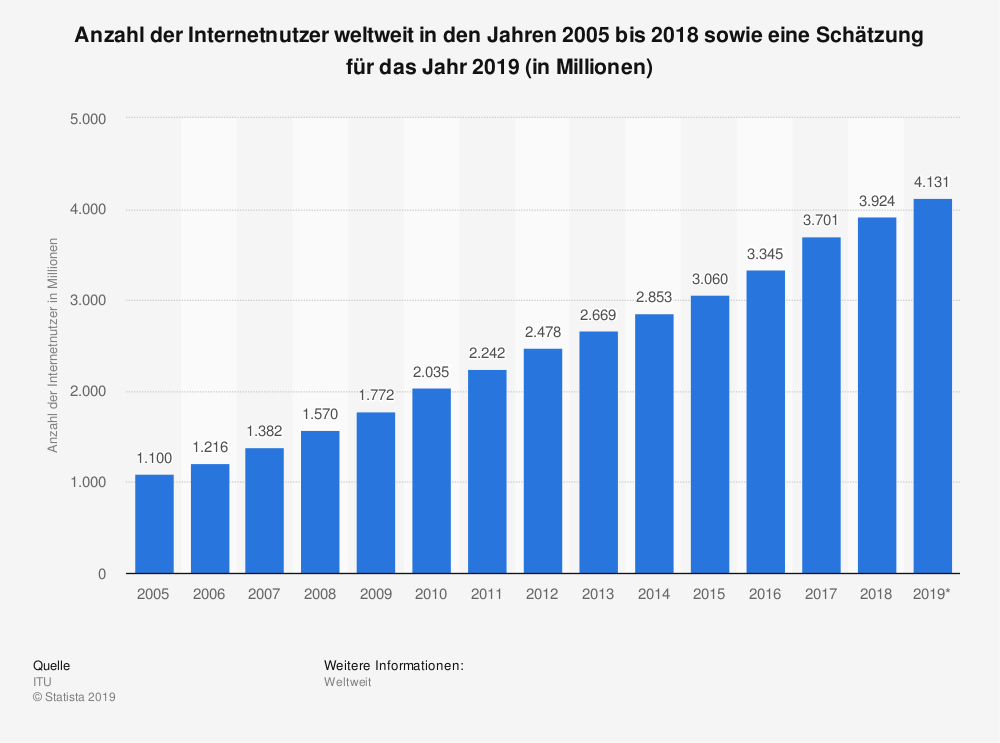
\includegraphics[width=0.7\textwidth]{stat}
\\
\cite[][27.03.2020]{Quelle: https://bit.ly/2TogWCc}
\end{figure}

Die IT Branche entwickelt sich stetig weiter. Das muss sie auch um mit dem steigenden Wachstum mithalten zu können.

Während einige Trends schnell in Vergessenheit geraten, etablieren sich wiederrum andere als solide Optionen in der Industrie.
Grundsätzlich muss jedes Unternehmnen abwägen ob es sich lohnt eine neue Software im Betrieb zu etablieren. Da dies immer mit Kosten verbunden ist, alleine als Zeitfaktor, 
will dies eine überlegte Investition sein.

Dazu sucht man sich Indikatoren an denen man messen kann ob eine Software nur ein Trend ist oder bestand hat. Solche Indikatoren wären zum Beispiel die Zukunftsaussicht der Lösung.
Wenn eine Software von einem annerkannten bekannten Unternehmen der Branche stamm, ist das Vertrauen natürlich ein anderes als wenn ein Startup oder eine Privatperson dahinter steht.
Auch das Alter der Software und Ehrfahrungsberichte von Unabhängigen haben ein großes Gewicht im Vergleich.

Kubernetes kann einige IT Prozesse im Unternehmen vereinfachen und automatisieren, was Kosten spart. Dennoch muss das Wissen erst aufgebaut werden, somit ist dies eine Rechnung die jedes Unternehmen
für sich machen muss. Die Frage ist nach dem ROI, dem Return-of-investment.

Was die Indikatoren angeht, kann man sagen das K8s dort sehr gut abschneidet. Wie erwähnt ist das Projekt von Google gestartet und wird seit je her auch von ihnen weiterentwickelt.
Man weiß das Google Kubernetes für ihre eigenen Services einsetzt, und auch K8s als Managed Service, als Software as a Service (Saas) Lösung in ihrer Cloud Platform anbietet.
Darüber hinaus setzen sehr viele der großen Unternehmen auf die K8s Platform, wie z.B. AirBnB und Reddit. Man kann also davon ausgehen, das die meisten dieser Unternehmen an
der Weiterentwicklung von K8s interessiert sind. Somit ist der Fortbestand kein Problempunkt.

Auch auf der Seite der Erfahrungsberichte kann Kubernetes punkten. Kubernetes würde nicht so viel Verwendung finden würden die Unternehmen darin nicht einen Vorteil sehen.
Natürlich macht K8s nicht in jeder Umgebung Sinn. Jeder muss abwägen wie er seine Infrastruktur aufbaut. Wenn man weiß das sie aber auf dauer stetig wachsen wird,
und man auf Punkte wie Hochverfügbarkeit setzen möchte, sollte Kubernetes auf jeden Fall eine Option sein die angeschaut werden sollte.

%-----------------------------------
% Anhang
%-----------------------------------
\newpage
\section*{Anhang} %Überschrift "Anhang", ohne Nummerierung
\addcontentsline{toc}{section}{\langde{Anhang}\langen{Appendix}} %Den Anhang ohne Nummer zum Inhaltsverzeichnis hinzufügen
\begin{appendices}
\addtocontents{toc}{\protect\setcounter{tocdepth}{0}} %
	\renewcommand{\thesection}{\langde{Anhang}\langen{Appendix} \arabic{section}:}
	\renewcommand\thesubsection{\langde{Anhang}\langen{Appendix} \arabic{section}.\arabic{subsection}:}
	%\section{Beispielanhang}\label{Beispielanhang}
%Dieser Abschnitt dient nur dazu zu demonstrieren, wie ein Anhang aufgebaut seien kann.
%\subsection{Weitere Gliederungsebene}
%Auch eine zweite Gliederungsebene ist möglich.
%\section{Bilder}
%Auch mit Bildern.
%Diese tauchen nicht im Abbildungsverzeichnis auf.
%\begin{figure}[H]
%    \centering
%    \caption[]{Beispielbild}
%	\label{fig:Beispielbild}
%    \includegraphics[width=1\textwidth]{verzeichnisStruktur}
%\end{figure}
\end{appendices}
\addtocontents{toc}{\protect\setcounter{tocdepth}{2}}

%-----------------------------------
% Literaturverzeichnis
%-----------------------------------
\newpage
%\addcontentsline{toc}{section}{Literatur}

% Die folgenden beiden Befehle würden ab dem Literaturverzeichnis wieder eine
% römische Seitennummerierung nutzen.
% Das ist nach dem Leitfaden nicht zu tun. Dort steht nur dass 'sämtliche
% Verzeichnisse VOR dem Textteil' römisch zu nummerieren sind. (vgl. S. 3)
%\pagenumbering{Roman} %Zähler wieder römisch ausgeben
%\setcounter{page}{4}  %Zähler manuell hochsetzen

% Ausgabe des Literaturverzeichnisses

% Keine Trennung der Werke im Literaturverzeichnis nach ihrer Art
% (Online/nicht-Online)
%\begin{RaggedRight}
%\printbibliography
%\end{RaggedRight}

% Alternative Darstellung, die laut Leitfaden genutzt werden sollte.
% Dazu die Zeilen auskommentieren und folgenden code verwenden:

% Literaturverzeichnis getrennt nach Nicht-Online-Werken und Online-Werken
% (Internetquellen).
% Die Option nottype=online nimmt alles, was kein Online-Werk ist.
% Die Option heading=bibintoc sorgt dafür, dass das Literaturverzeichnis im
% Inhaltsverzeichnis steht.
% Es ist übrigens auch möglich mehrere type- bzw. nottype-Optionen anzugeben, um
% noch weitere Arten von Zusammenfassungen eines Literaturverzeichnisse zu
% erzeugen.
% Beispiel: [type=book,type=article]
\printbibliography[nottype=online,heading=bibintoc,title={\langde{Literaturverzeichnis}\langen{Bibliography}}]

% neue Seite für Internetquellen-Verzeichnis
\newpage

% Laut Leitfaden 2018, S. 14, Fussnote 44 stehen die Internetquellen NICHT im
% Inhaltsverzeichnis, sondern gehören zum Literaturverzeichnis.
% Die Option heading=bibintoc würde die Internetquelle als eigenen Eintrag im
% Inhaltsverzeicnis anzeigen.
%\printbibliography[type=online,heading=bibintoc,title={Internetquellen}]
\printbibliography[type=online,title={\langde{Internetquellen}\langen{Internet sources}}]

\newpage
\pagenumbering{gobble} % Keine Seitenzahlen mehr

%-----------------------------------
% Ehrenwörtliche Erklärung
%-----------------------------------
\section*{
	\langde{Ehrenwörtliche Erklärung}
	\langen{Declaration in lieu of oath}}
\langde{Hiermit versichere ich, dass die vorliegende Arbeit von mir selbstständig und ohne unerlaubte Hilfe angefertigt worden ist, insbesondere dass ich alle Stellen, die wörtlich oder annähernd wörtlich aus Veröffentlichungen entnommen sind, durch Zitate als solche gekennzeichnet habe. Weiterhin erkläre ich, dass die Arbeit in gleicher oder ähnlicher Form noch keiner Prüfungsbehörde/Prüfungsstelle vorgelegen hat. Ich erkläre mich damit einverstanden, dass die Arbeit der Öffentlichkeit zugänglich gemacht wird. Ich erkläre mich damit einverstanden, dass die Digitalversion dieser Arbeit zwecks Plagiatsprüfung auf die Server externer Anbieter hochgeladen werden darf. Die Plagiatsprüfung stellt keine Zurverfügungstellung für die Öffentlichkeit dar.}
\langen{I hereby declare that I produced the submitted paper with no assistance from any other party and without the use of any unauthorized aids and, in particular, that I have marked as quotations all passages which are reproduced verbatim or near-verbatim from publications. Also, I declare that the submitted print version of this thesis is identical with its digital version. Further, I declare that this thesis has never been submitted before to any examination board in either its present form or in any other similar version. I herewith agree/disagree that this thesis may be published. I herewith consent that this thesis may be uploaded to the server of external contractors for the purpose of submitting it to the contractors’ plagiarism detection systems. Uploading this thesis for the purpose of submitting it to plagiarism detection systems is not a form of publication.}


\par\medskip
\par\medskip

\vspace{5cm}

\begin{table}[H]
	\centering
	\begin{tabular*}{\textwidth}{c @{\extracolsep{\fill}} ccccc}
		\myOrt, \the\day.\the\month.\the\year
		&
		% Hinterlege deine eingescannte Unterschrift im Verzeichnis /abbildungen und nenne sie unterschrift.png
		% Bilder mit transparentem Hintergrund können teils zu Problemen führen
		
\includegraphics[width=0.35\textwidth]{unterschrift}\vspace*{-0.35cm}
		\\
		\rule[0.5ex]{12em}{0.55pt} & \rule[0.5ex]{12em}{0.55pt} \\
		\langde{(Ort, Datum)}\langen{(Location, Date)} & \langde{(Eigenhändige Unterschrift)}\langen{(handwritten signature)}
		\\
	\end{tabular*} \\
\end{table}

\end{document}
